\documentclass{beamer}

\usepackage{amsfonts}
\usepackage{amsmath}
\usepackage{longtable}
\usepackage{csquotes}
\usepackage{standalone}

\usepackage{graphicx}
\graphicspath{{../pictures/}}

\usepackage{tikz}
\usetikzlibrary{shapes, calc, arrows, decorations.markings,
  decorations.pathmorphing, decorations, patterns, chains, snakes,
  backgrounds, positioning, fit, petri}
\newcommand{\inputpicture}[1]{\input{../drawings/#1}}

\usepackage{listings}
\lstset{language=C, basicstyle=\ttfamily, breaklines=true, keepspaces=true,
  keywordstyle=\color{blue}}

\usepackage{bytefield}

\usefonttheme{professionalfonts}
\usefonttheme{serif}
\usepackage{fontspec}
\setromanfont{CMU Serif}
\setsansfont{CMU Sans Serif}
\setmonofont{CMU Typewriter Text}

\usepackage{hyperref}
\hypersetup{colorlinks=true, linkcolor=black, filecolor=black, citecolor=black,
  urlcolor=blue , pdfauthor=Evgenii Iuliugin <yulyugin@gmail.com>,
  pdftitle=Fundamentals of Full-Platform Simulation}

\usepackage{underscore}
\usepackage{amsthm}

\subtitle{Fundamentals of Full-Platform Simulation}
\subject{Lecture}
\date{\today}

\author[Evgenii Iuliugin]{
  Evgenii Iuliugin \small{\href{mailto:yulyugin@gmail.com}{yulyugin@gmail.com}}}
\typeout{Copyright 2021 Evgenii Iuliugin}

\usetheme{Berlin}
\setbeamertemplate{navigation symbols}{}

\newcommand{\finalslide}{
    {\huge{Thank you!}\par}

    \vfill
    Slides and material are available at
    \url{https://github.com/yulyugin/sim-lectures}
    \vfill

    \tiny{\textit{Note}: All trademarks are the property of their respective
        owners.
        The presented point of view reflects the personal opinion of the author.

        %All the materials are licensed under the Creative Commons
        %Attribution-NonCommercial-ShareAlike 4.0 Worldwide. To view a copy of
        %this license, visit
        %\url{http://creativecommons.org/licenses/by-nc-sa/4.0/}.
    }
}


\title{Simulation Role in Software and Hardware Development}

\begin{document}

\startslides

\section{Complexity of Modern Computer Systems}

\begin{frame}{Complexity of Modern Computer Systems}

\centering
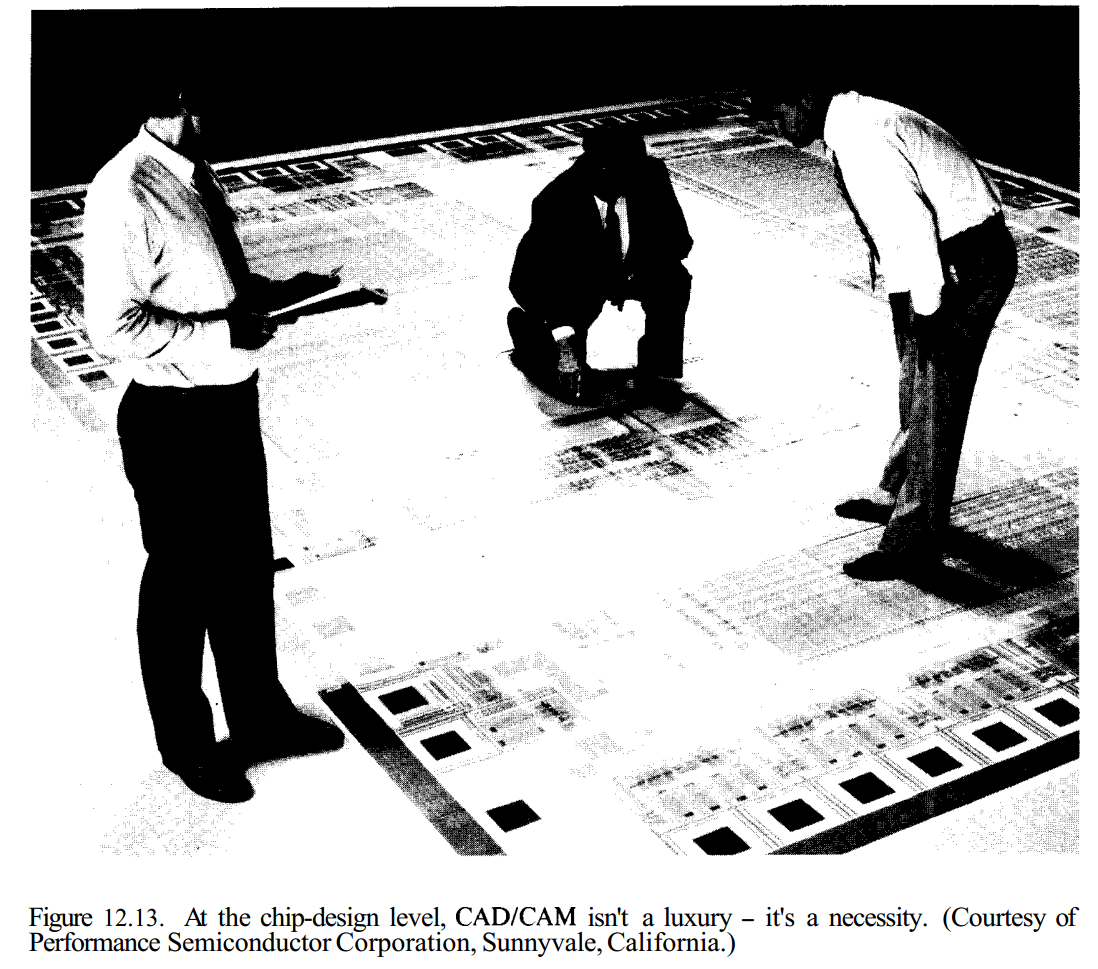
\includegraphics[width=0.7\textwidth]{ic-floor}

\tiny{Source: P. Horowitz and W. Hill. 1989. The Art of Electronics. Cambridge
University Press, New York, NY, USA}

\end{frame}

\begin{frame}{Why Software Development Only On Real Hardware Is Not Beneficial?}

\begin{itemize}
\item Amount of available samples is usually limited,
\item low-level debug is challenging,
\item long development cycle.
\end{itemize}

$\Rightarrow$ development cost is increasing.

\bigskip

``\tiny{I've noticed a shift during the past couple of years towards an increasing
use of various types of simulation, including virtual platforms. Previously
software developers wanted real hardware, but now they have to start using
simulation because there's no chip available.``
\textit{Tomas Evensen, Wind River CTO}}

\end{frame}

\begin{frame}{Solution --- Software Models of Real Hardware}
\centering 
\inputpicture{idea}

\end{frame}

\section{Areas of Application}

\begin{frame}{Areas of Application}

\pause
\begin{itemize}
\item New hardware development,
\item software and hardware co-development,
\item experimental architectures,
\item power and performance prediction,
\item compatibility with other architecures.
\end{itemize}

\end{frame}

\begin{frame}{New Hardware Development}

\inputpicture{error-cost}

\end{frame}

\begin{frame}{Software and Hardware Development}

\pause
\begin{itemize}
\item Firmware, BIOS, UEFI.
\item Operation systems.
\item Device drivers.
\item Compilers.
\item Applications.
\end{itemize}

\end{frame}

\begin{frame}{``Shift Left`` --- Accelerated Product Development}

\centering

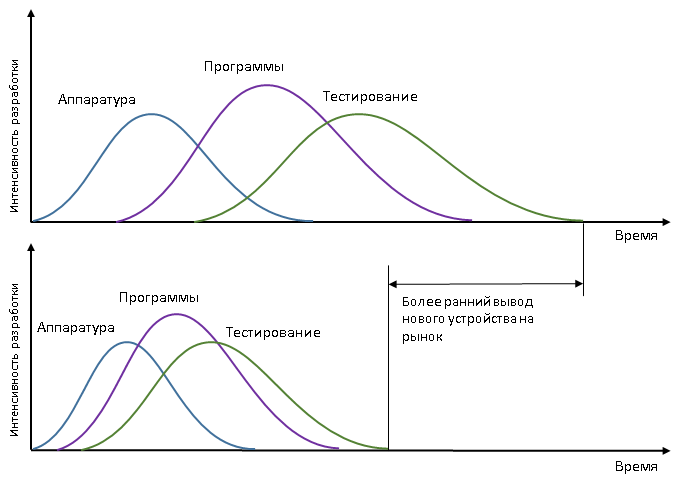
\includegraphics[width=1\textwidth]{shift-left} % TODO TikZ-elize this

\begin{tiny}
Impact of Shift left on hardware/software development.
Source: Semiconductor Engineering
\end{tiny}

\vfill

\begin{itemize}
\item Allow early software development --- before silicon arrives.
\item Shorten time to marked by overlapping hardware and software designs.
\item Decouple software and hardware development.
\item Validation of software, hardware, and their integration starts earlier.
\end{itemize}

\end{frame}

\begin{frame}{Experimental Architectures}

\begin{itemize}
\item New Instruction Set Architectures (ISA).
\item New ISA extensions.
\item Multicore systems.
\item Vector systems.
\item Security and Cryptography.
\end{itemize}

\end{frame}

\begin{frame}{Power and Performance Prediction}

\begin{itemize}
\item Untimed,
\item Loosely Timed,
\item Approximately timed.
\end{itemize}

\end{frame}

\begin{frame}{Compatibility with Other Architectures}
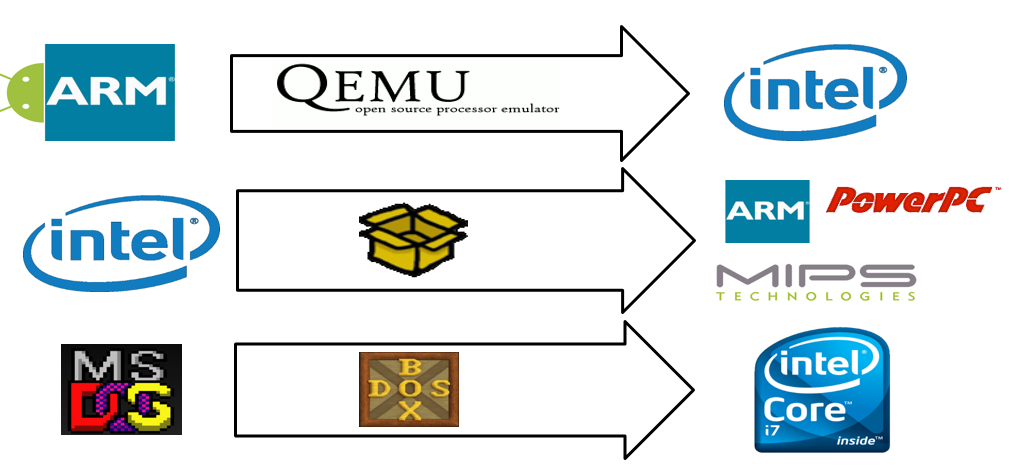
\includegraphics[width=\textwidth]{compat} % TODO TikZ-elize this
\end{frame}

\section{Terminology}

\begin{frame}{Terminology}
\begin{itemize}
\item \textbf{Simulation} --- replication of system's behavior that can be
      observed through \textbf{\textit{external}} interaction with the system.
\item \textbf{Emulation} --- replication of a system's behavior considering how
      the system \textbf{\textit{internally}} works through imitation of all
      internal structures and processes.
\item \textbf{Virtualization} --- effective isolation of several systems from
      each other with simultaneous and transparent access to resources of the
      underlying system.
\end{itemize}

\end{frame}

\begin{frame}{Types of Simulators}
\begin{itemize}
\item Full-platform,
\item Application level,
\item Functional,
\item Cycle-accurate,
\item Software,
\item Hybrid.
\end{itemize}
\end{frame}

\begin{frame} {Terminology}
\begin{itemize}
\item Host,
\item Guest, target.
\end{itemize}
\end{frame}

\section{Capabilities}

\begin{frame}{Some Simulation Capabilities}
\begin{itemize}
\item Non-intrusive inspection,
\item Repeatability,
\item Save/restore of simulated state,
\item Synchronized system stop,
\item Reverse execution.
\end{itemize}
\end{frame}

\section{Conclusions}

\begin{frame}{Conclusions}
\begin{itemize}
\item Software models are created before hardware availability.
\item Software models are used for software-hardware co-development.
\item Simulation provides unique debugging and development capabilities.
\end{itemize}
\end{frame}

\begin{frame}[allowframebreaks]{Bibliography}
\begin{thebibliography}{99}
  \bibitem{} [RUS] \textit{Речистов~Г.С, Юлюгин~Е.А и др.},
    Программное моделирование вычислительных систем.
    \url{https://github.com/grigory-rechistov/simbook/blob/master/metoda/main-web.pdf}
  \bibitem{} \textit{James Smith, Ravi Nair}, Virtual machines -- Versatile
    Platforms for Systems and Processes.
\end{thebibliography}
\end{frame}

\begin{frame}{On the next lecture:}
\begin{itemize}
\item Terminology,
\item general requirements for simulation.
\end{itemize}
\end{frame}

\finalslide

\end{document}
